\chapter[Even Representations, Torsion and Potential Modularity]{Even Representations, Torsion\\ and Potential Modularity:\\ Calegari's Theorems in Thorin Form}\label{ch:cal}

The frontier of reciprocity in dimension two is drawn by a handful of theorems of the last fifteen years, and Frank Calegari is an author of most of them. Even two dimensional geometric Galois representations with distinct Hodge Tate weights do not exist, under mild hypotheses, so that the Fontaine Mazur conjecture holds for them vacuously and the even representations that remain are conjecturally those of Artin type, the ones Chapter~\ref{ch:maass} placed among the Maass forms of eigenvalue $\frac14$ (Calegari \cite{calegari2011,calegari2012}). Modularity lifting can be pushed past the Taylor Wiles method into the situations where the relevant cohomology lives in several degrees and carries torsion, which over $\Q$ is weight one and over other number fields is the Betti cohomology of locally symmetric spaces (Calegari and Geraghty \cite{calegarigeraghty2018}). Elliptic curves over CM fields are potentially modular, satisfy the Sato Tate conjecture, and the Ramanujan conjecture holds for weight zero forms over such fields (Allen, Calegari, Caraiani, Gee, Helm, Le Hung, Newton, Scholze, Taylor and Thorne \cite{accghlnstt2023}). Abelian surfaces over totally real fields are potentially modular, so that the Hasse Weil $L$ function of every genus two curve over $\Q$ has meromorphic continuation and a functional equation (Boxer, Calegari, Gee and Pilloni \cite{bcgp2021}). And the torsion in the cohomology of arithmetic groups, which the Taylor Wiles method cannot see, is governed by analytic torsion and satisfies its own Jacquet Langlands correspondence (Calegari and Venkatesh \cite{calegarivenkatesh2019}, Bergeron and Venkatesh \cite{bergeronvenkatesh2013}).

This chapter reads these theorems in the dictionary of the book and records what each one gives back. The first yields a new theorem: the comparison of the two gamma factors in the Galois heat trace of Chapter~\ref{ch:recip}, which Section~\ref{sec:msquarter} makes in weight one, holds in every weight, with the hyperbolic secant law replaced by its convolution with a Cauchy law whose scale is half the weight, and Calegari's theorem then says that for distinct Hodge Tate weights only one of the two archimedean terms is ever realised. The third makes the Dirichlet process of Chapter~\ref{ch:pd} a theorem over every CM field with the Sato Tate law as base measure, and makes the local Thorin positivity of Chapter~\ref{ch:maass} unconditional for weight zero forms over such fields; a curve over $\Q(i)$ is checked at $664581$ primes. The fourth makes the Thorin equivalence of Chapter~\ref{ch:10b} a well posed statement for abelian surfaces, and a genus two curve of conductor $249$ is checked against its zeros. The last connects the torsion growth of Bergeron and Venkatesh to the entropy theorem of Chapter~\ref{ch:hit}, and leaves an open problem.

\section*{Contributions of this chapter}

\begin{enumerate}
\item[(1)] \emph{Parity in every weight} (Theorem~\ref{thm:calparity}). For Hodge Tate weights $(0,w)$ the heat traces with the holomorphic gamma factor $\Gamma_\C(s+\frac w2)$ and the even gamma factor $\Gamma_\R(s+\frac w2)^2$ differ by $\Delta_w(x)=\frac14\E e^{-xC_w^2}$, $C_w=C+\frac w2T$, the hyperbolic secant variable plus an independent Cauchy variable of scale $w/2$. The weight one case of Chapter~\ref{ch:flt} is $w=0$. Under GRH an odd representation has a completely monotone heat trace with the holomorphic factor and not with the even one, the defect being $\frac14f_w(0)\sqrt{\pi/x}$; checked for $11a1$ with $388$ zeros.
\item[(2)] \emph{Calegari's theorem read in the heat trace} (Section~\ref{sec:calparity}). For geometric two dimensional representations with distinct Hodge Tate weights only the holomorphic archimedean term is ever realised; the heat trace decides the parity exactly in the one case, $w=0$, where Calegari's theorem does not apply.
\item[(3)] \emph{The Dirichlet process over CM fields} (Theorem~\ref{thm:calcm}). For an elliptic curve without complex multiplication over a CM field, the labelled factorisation of the $\zeta_F$ random ideal converges to the Dirichlet process with Sato Tate base measure, and every Frobenius functional to a GGC with the Sato Tate image as Thorin measure; this was conditional before \cite{accghlnstt2023}. Checked for $y^2=x^3+ix+1$ over $\Q(i)$ at $664581$ primes.
\item[(4)] \emph{Local Thorin positivity for Bianchi forms} (Corollary~\ref{cor:calbianchi}). The local factors of weight zero cuspidal representations over CM fields are GGC transforms in $\sqrt\lambda$ with explicit Thorin combs, unconditionally, by the Ramanujan theorem of \cite{accghlnstt2023}, which over CM fields has no Shimura variety behind it; the corresponding statement over $\Q$ for Maass forms of eigenvalue $\frac14$, which are not cohomological, is open.
\item[(5)] \emph{The Thorin criterion for abelian surfaces} (Theorem~\ref{thm:calg2}). After \cite{bcgp2021} the function $\Xi_A(0)/\Xi_A(\sqrt\lambda)$ exists as a meromorphic function for every abelian surface over $\Q$, is entire for the modular ones, and GRH for $A$ is its membership in the GGC class; the shifted representation at basepoints $1+a$, $a\ge\frac12$, is unconditional. Checked for the genus two curve of conductor $249$ against its zeros, with the $\USp(4)$ Frobenius moments.
\item[(6)] \emph{Torsion growth and tree entropy} (Section~\ref{sec:caltorsion}). The torsion growth of Bergeron and Venkatesh and the entropy theorem of Chapter~\ref{ch:hit} are the archimedean and $p$ adic cases of one statement about Jacquet Langlands invariant growth rates computed from return probabilities on the universal cover; the identification of the constants is posed as Open Problem~\ref{op:caltorsion}.
\item[(7)] Four open problems and a computational problem: parity without GRH, the Gamma shape and Euler Kronecker drift over CM fields, Sato Tate for abelian surfaces as a Dirichlet process, and the torsion entropy.
\end{enumerate}

\section{The theorems}\label{sec:calthm}

Throughout, $\rho:\Gal(\overline\Q/\Q)\to\GL_2(\overline{\Q}_p)$ is continuous and unramified outside finitely many primes, $c$ is a complex conjugation, and $\rho$ is \emph{odd} if $\det\rho(c)=-1$ and \emph{even} if $\det\rho(c)=1$. Modular representations are odd, because complex conjugation acts on the cohomology of a modular curve with eigenvalues $1$ and $-1$ on each two dimensional Hecke eigenspace. The Fontaine Mazur conjecture \cite{fontainemazur1995} predicts that every irreducible odd $\rho$ that is de Rham at $p$ comes, up to twist, from a modular form, and for even $\rho$ it predicts that the de Rham ones have finite image up to twist. Calegari's theorem is the even half of this in the case of distinct Hodge Tate weights.

\begin{theorem}[Calegari \cite{calegari2011}]\label{thm:caleven}
Let $p>7$ and let $\rho$ be irreducible with residual image containing $\SL_2(\mathbb F_p)$. Suppose $\rho$ is ordinary at $p$ with distinct Hodge Tate weights. Then $\rho$ is odd, and is modular.
\end{theorem}

Oddness, though not modularity, is proved in the same way over totally real fields $E$ with $[E(\zeta_p)^+:E]>2$, and the sequel \cite{calegari2012} removes the ordinarity hypothesis under similar conditions. Some $p$ adic Hodge theory hypothesis is necessary: Ramakrishna \cite{ramakrishna2002} constructed even representations with image $\SL_2(\Z_7)$ unramified outside a finite set, which are therefore not de Rham. The proof of Theorem~\ref{thm:caleven} is a potential modularity argument, in Calegari's own summary: $\rho$ becomes modular over some totally real field, and modular representations are odd; the actual route is through the potential automorphy of the adjoint representation and a descent. The companion statement over imaginary quadratic fields says that, under similar hypotheses, a geometric representation over such a field whose two Hodge Tate weights at the two places above $p$ are $(0,m)$ and $(0,n)$ must have $m=n$.

The even representations that survive are those with equal Hodge Tate weights, which, conjecturally, are after a twist the Artin representations of Chapter~\ref{ch:03}, and the automorphic objects on their side are the Maass forms of eigenvalue $\frac14$ (Section~\ref{sec:msquarter}). The Taylor Wiles method does not reach them. Its numerology requires the automorphic forms in question to contribute to a single degree of torsion free cohomology; weight one forms contribute to the coherent cohomology of modular curves in two degrees, and over general number fields the Betti cohomology of the locally symmetric space is spread over several degrees and carries torsion, while Maass forms of eigenvalue $\frac14$ contribute to no cohomology at all, which is why even Artin representations are the hardest case. Calegari and Geraghty \cite{calegarigeraghty2018} showed how to run the method when the cohomology is spread and has torsion: unconditionally in weight one over $\Q$, where they identify deformation rings with Hecke algebras acting on $p$ adic weight one forms, and in general conditionally on the existence of Galois representations attached to torsion classes in the cohomology of locally symmetric spaces. Under that conjecture every elliptic curve over every number field would be potentially modular and satisfy Sato Tate.

Over CM fields enough of the conjecture was established, through the Galois representations attached to torsion classes by Scholze and the vanishing theorems of Caraiani and Scholze, for the method to go through.

\begin{theorem}[Allen, Calegari, Caraiani, Gee, Helm, Le Hung, Newton, Scholze, Taylor and Thorne \cite{accghlnstt2023}]\label{thm:calcmfield}
Let $F$ be a CM field. Every elliptic curve over $F$ is potentially modular and satisfies the Sato Tate conjecture. Every cuspidal automorphic representation of $\GL_2(\A_F)$ of weight zero, that is cohomological for the trivial coefficient system, is tempered at every finite place; in particular it satisfies the Ramanujan conjecture at every unramified place.
\end{theorem}

\begin{theorem}[Boxer, Calegari, Gee and Pilloni \cite{bcgp2021}]\label{thm:calbcgp}
Every abelian surface over a totally real field is potentially modular. Consequently the Hasse Weil $L$ function of every genus two curve over a totally real field has meromorphic continuation to $\C$ and satisfies the expected functional equation. Infinitely many abelian surfaces over $\Q$ with geometric endomorphism ring $\Z$, pairwise non isogenous even up to twist, are modular.
\end{theorem}

The torsion results are stated in Section~\ref{sec:caltorsion}.

\section{Parity in every weight}\label{sec:calparity}

Section~\ref{sec:msquarter} shows that for a two dimensional Artin representation the parity is visible in the heat trace of Theorem~\ref{thm:recipcm}: the archimedean term built with $\Gamma_\C(s)$, the gamma factor of weight one, and the one built with $\Gamma_\R(s)^2$, the gamma factor of a Maass form of eigenvalue $\frac14$, differ by $\Delta(x)=\frac14\E e^{-xC^2}$ with $C$ hyperbolic secant distributed, and under GRH the heat trace is completely monotone with the right gamma factor and not with the wrong one. That is the case of Hodge Tate weights $(0,0)$. Calegari's theorem concerns weights $(0,w)$ with $w>0$, where the holomorphic gamma factor is $\Gamma_\C(s+\frac w2)$, the gamma factor of weight $k=w+1$, and the candidate even gamma factor is $\Gamma_\R(s+\frac w2)^2$. The comparison extends to this case with an explicit law.

\begin{theorem}[parity from positivity in every weight; this book]\label{thm:calparity}
Let $\rho$ be self dual with $\Lambda(s,\rho)=\Lambda(1-s,\rho)$, and for $w\ge0$ let $\mathcal W^{\mathrm{hol}}_\rho$ and $\mathcal W^{\mathrm{ev}}_\rho$ be the heat traces of Definition~\ref{def:recipheat} computed with the gamma factors $\Gamma_\C(s+\frac w2)=\Gamma_\R(s+\frac w2)\Gamma_\R(s+\frac w2+1)$ and $\Gamma_\R(s+\frac w2)^2$ respectively, the same conductor and the same Frobenius data.
\begin{enumerate}
\item[(a)] Unconditionally,
\begin{gather*}
\mathcal W^{\mathrm{hol}}_\rho(x)-\mathcal W^{\mathrm{ev}}_\rho(x)=\Delta_w(x):=\frac14\E e^{-xC_w^2},\\
\Delta_w(x)=\frac1{4\sqrt{\pi x}}\int_0^\infty\frac{e^{-wu/2}}{\cosh(u/2)}\,e^{-u^2/4x}\,du,
\end{gather*}
where $C_w=C+\frac w2\,T$ with $C$ hyperbolic secant distributed, density $\operatorname{sech}(\pi t)$, and $T$ an independent standard Cauchy variable. So $\Delta_w$ is completely monotone, and $\Delta_w(x)\sim\frac14f_w(0)\sqrt{\pi/x}$ as $x\to\infty$, where
\[
f_w(0)=\int_\R\operatorname{sech}(\pi s)\,\frac{w/2\pi}{(w/2)^2+s^2}\,ds
\]
is the density of $C_w$ at $0$; $f_w(0)=1$, $0.4413$, $0.1953$, $0.0574$ for $w=0,1,3,11$. For $w=0$ the Cauchy factor is a point mass at $0$ and $f_0(0)=\operatorname{sech}0=1$ is read as the limit $w\to0$.
\item[(b)] Suppose $\Lambda(s,\rho)$ is entire with root number $+1$ and satisfies GRH, and that $\rho$ is odd with Hodge Tate weights $(0,w)$, so that its gamma factor is $\Gamma_\C(s+\frac w2)$. Then $\mathcal W^{\mathrm{hol}}_\rho=\frac12\sum e^{-x\gamma^2}$ over the zeros is completely monotone, and $\mathcal W^{\mathrm{ev}}_\rho$ is not: $\mathcal W^{\mathrm{ev}}_\rho(x)-\mathcal W^{\mathrm{ev}}_\rho(\infty)\sim-\frac14f_w(0)\sqrt{\pi/x}$ is negative and increasing at infinity.
\end{enumerate}
\end{theorem}

\begin{proof}
(a) The two heat traces share the conductor and the prime sum, so their difference is the archimedean term, $\frac1{4\pi}\int_\R e^{-xt^2}\,2\operatorname{Re}[\gamma'_{\mathrm{hol}}/\gamma_{\mathrm{hol}}-\gamma'_{\mathrm{ev}}/\gamma_{\mathrm{ev}}](\tfrac12+it)\,dt$. With $\Gamma_\R'/\Gamma_\R(s)=\frac12\psi(s/2)-\frac12\log\pi$ and $z=\frac12+\frac w2+it$ the bracket is $\operatorname{Re}[\psi(\frac{z+1}2)-\psi(\frac z2)]$, and the integral representation
\[
\psi\Bigl(\frac{z+1}2\Bigr)-\psi\Bigl(\frac z2\Bigr)=2\int_0^\infty\frac{e^{-zu}}{1+e^{-u}}\,du,\qquad\operatorname{Re}z>0,
\]
gives
\[
\operatorname{Re}\Bigl[\psi\Bigl(\tfrac{z+1}2\Bigr)-\psi\Bigl(\tfrac z2\Bigr)\Bigr]=\int_0^\infty\frac{2e^{-(w+1)u/2}\cos(tu)}{1+e^{-u}}\,du=\int_0^\infty\frac{e^{-wu/2}\cos(tu)}{\cosh(u/2)}\,du .
\]
Integrating against $e^{-xt^2}$ with $\int_\R e^{-xt^2}\cos(tu)\,dt=\sqrt{\pi/x}\,e^{-u^2/4x}$ gives the first formula. For the second, let $h_w(u)=e^{-w|u|/2}\operatorname{sech}(u/2)$, even with $h_w(0)=1$, so that $\hat h_w(t)/2\pi$ is a probability density, the law of $C_w$; by Parseval $\frac1{8\sqrt{\pi x}}\int_\R h_w(u)e^{-u^2/4x}du=\frac1{8\pi}\int_\R e^{-xt^2}\hat h_w(t)\,dt=\frac14\E e^{-xC_w^2}$. The Fourier transform of $\operatorname{sech}(u/2)$ is $2\pi\operatorname{sech}(\pi t)$ and that of $e^{-w|u|/2}$ is $w/((w/2)^2+t^2)$, so $\hat h_w/2\pi$ is the convolution of the secant density with the Cauchy density of scale $w/2$, which is the law of $C+\frac w2T$. The integrand is positive, so $\Delta_w>0$, complete monotonicity is Bernstein's theorem, and the asymptotic is Laplace's method at the density's value at $0$.

(b) The first statement is Theorem~\ref{thm:recipcm} for the gamma factor of $\rho$. For the second, $\mathcal W^{\mathrm{ev}}=\mathcal W^{\mathrm{hol}}-\Delta_w$, and $\mathcal W^{\mathrm{hol}}(x)-\mathcal W^{\mathrm{hol}}(\infty)=\frac12\sum_{\gamma\ne0}e^{-x\gamma^2}$ decays exponentially while $\Delta_w$ decays like $x^{-1/2}$; a completely monotone function is decreasing.
\end{proof}

For $w=0$ this is the comparison of Section~\ref{sec:msquarter}. For the curve $11a1$, $w=1$, the heat trace from the $388$ zeros below height $300$ with the tail from the zero counting function gives $\mathcal W^{\mathrm{hol}}=0.916$, $0.165$, $0.0181$, $3\cdot10^{-4}$, $2\cdot10^{-9}$ at $x=0.02$, $0.05$, $0.1$, $0.2$, $0.5$, decreasing to $0$ as a completely monotone function with no zero at the centre must, while $\mathcal W^{\mathrm{ev}}=\mathcal W^{\mathrm{hol}}-\Delta_1$ equals $0.685$, $-0.054$, $-0.189$, $-0.190$, $-0.163$, $-0.137$, $-0.058$, $-0.027$ at $x=0.02$, $0.05$, $0.1$, $0.2$, $0.5$, $1$, $10$, $50$, crossing zero and then increasing to $0$ from below at the rate $0.196/\sqrt x$ (Figure~\ref{fig:calparity}). The closed form of $\Delta_w$ was checked against the direct archimedean integral to $10^{-16}$ at twelve values of $(w,x)$.

\begin{figure}[t]
\centering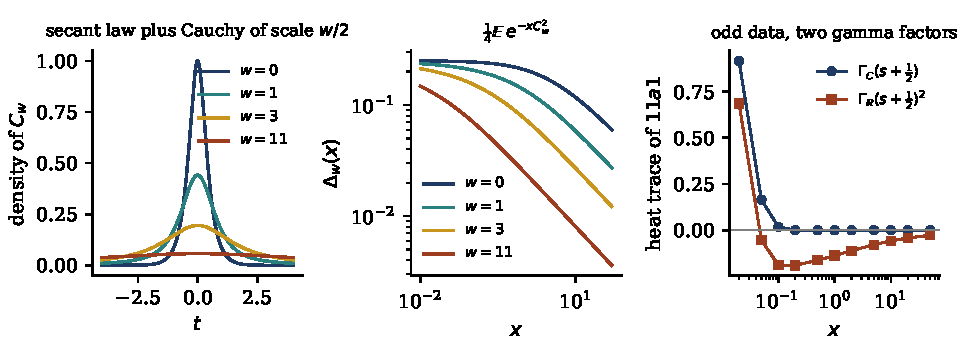
\includegraphics[width=\textwidth]{figs/cal_parity.pdf}
\caption{Parity in every weight. Left: the densities of $C_w=C+\frac w2T$ for $w=0,1,3,11$, the secant law convolved with a Cauchy law of scale $w/2$. Centre: $\Delta_w(x)=\frac14\E e^{-xC_w^2}$. Right: the heat trace of $11a1$ with the holomorphic gamma factor $\Gamma_\C(s+\frac12)$, completely monotone, and with the even gamma factor $\Gamma_\R(s+\frac12)^2$, which crosses zero and increases.}\label{fig:calparity}
\end{figure}

Calegari's theorem now reads as follows. A geometric representation with distinct Hodge Tate weights $(0,w)$ is assigned, by the motivic recipe, the gamma factor $\Gamma_\C(s+\frac w2)$ whatever its parity, and this is the gamma factor of the discrete series representation of $\GL_2(\R)$ of weight $w+1$, which is odd; the even factors $\Gamma_\R(s+\frac w2)^2$ and $\Gamma_\R(s+\frac w2+1)^2$ belong to archimedean parameters with equal exponents, that is to weights $(\frac w2,\frac w2)$, and are realised by no automorphic representation with weights $(0,w)$. They are the candidates against which the heat trace is tested. Theorem~\ref{thm:caleven} says that under its hypotheses the even case does not arise, and Theorem~\ref{thm:calparity} says what the heat trace sees: the archimedean term that makes the Frobenius data of a geometric $\rho$ with distinct weights a Laplace transform is the holomorphic one, and the even one misses by exactly $\Delta_w$. At $w=0$ both archimedean terms are realised, by weight one forms and by Maass forms of eigenvalue $\frac14$, and the heat trace decides between them; for $w>0$ Calegari's theorem removes the choice. The motivic reason is simple: on a motive with Hodge numbers $h^{0,w}=h^{w,0}=1$ and $w>0$, complex conjugation swaps the two Hodge pieces and so has eigenvalues $1$ and $-1$; what Calegari proves is that geometric representations behave as motives in this respect, without knowing that they are motives.

\section{CM fields: the Dirichlet process with Sato Tate base measure}\label{sec:calcm}

Let $F$ be a CM field, $E/F$ an elliptic curve without complex multiplication, and for each prime $\mathfrak p$ of good reduction write $a_{\mathfrak p}=2\sqrt{N\mathfrak p}\cos\theta_{\mathfrak p}$. The Sato Tate statement of Theorem~\ref{thm:calcmfield} is that the $\theta_{\mathfrak p}$, ordered by norm, are equidistributed for the Sato Tate law $\frac2\pi\sin^2\theta\,d\theta$. Chapters~\ref{ch:recip} and \ref{ch:pd} built everything on an equidistribution hypothesis of exactly this kind, with the primes of $\Q$ replaced by the primes of $F$ and $\zeta$ by $\zeta_F$, and so they apply.

\begin{theorem}[the Dirichlet process over a CM field; this book]\label{thm:calcm}
Let $F$, $E$ be as above and let $\mathfrak n_\sigma$ be the random ideal of $F$ with $\Prob(\mathfrak n_\sigma=\mathfrak n)=N\mathfrak n^{-\sigma}/\zeta_F(\sigma)$, its prime factors labelled by $\theta_{\mathfrak p}$. As $\sigma\downarrow1$:
\begin{enumerate}
\item[(i)] the labelled factorisation converges in law to the Gamma process with label law Sato Tate, and the normalised factorisation to the Dirichlet process with base measure $\frac2\pi\sin^2\theta\,d\theta$;
\item[(ii)] for continuous $Q\ge0$ on $[0,\pi]$ the Frobenius functional $\Xi_\sigma(Q)=(\sigma-1)\sum_{\mathfrak p}e_{\mathfrak p}\log N\mathfrak p\,Q(\theta_{\mathfrak p})$ converges to the GGC with Thorin measure the image of the Sato Tate law under $1/Q$; for $Q=\cos^2$ the Thorin density is $\frac2{\pi t^2}\sqrt{t-1}$ on $(1,\infty)$;
\item[(iii)] the same holds with the labels $(\theta_{\mathfrak p},\Frob_{\mathfrak p})$ in $[0,\pi]\times G$ for any finite Galois extension $L/F$, with base measure the product of Sato Tate and Haar measure, the joint equidistribution following, as in Chapter~\ref{ch:04}, from the Weyl criterion with the $L$ functions $L(s,\Sym^mE\otimes\chi)$, $\chi$ an irreducible character of $\Gal(L/F)$, whose nonvanishing on $\operatorname{Re}s=1$ follows from the potential automorphy of all symmetric powers in \cite{accghlnstt2023} by Brauer induction and the theorem of Jacquet and Shalika.
\end{enumerate}
\end{theorem}

\begin{proof}
Lemma~\ref{lem:recipnu} and the proof of Theorem~\ref{thm:recipgammaproc} use the prime number theorem for the primes of $F$, which is Landau's prime ideal theorem, the bound $\sum_{\mathfrak p}N\mathfrak p^{-2}<\infty$, and the equidistribution of the labels, which is Theorem~\ref{thm:calcmfield}. Nothing else enters. (ii) is Theorem~\ref{thm:recipggcfun} and the Sato Tate image was computed in Section~\ref{sec:gl1cm}. (iii) is the same with the product labels, the joint equidistribution being supplied by the symmetric power $L$ functions twisted by the characters of $\Gal(L/F)$, exactly as the Sato Tate theorem itself is deduced from the untwisted ones.
\end{proof}

The curve $E:y^2=x^3+ix+1$ over $\Q(i)$, with $j$ invariant $(27648-186624i)/745$, not an algebraic integer, hence without complex multiplication, and conductor of norm $190720$, has $664581$ primes of norm at most $10^7$ above the rational primes not dividing the conductor, of which $225$ are the inert primes of residue degree two; the two good primes above $5$ and $149$ were left out with the bad ones. The normalised traces have moments $0.9988$, $1.9957$, $4.9842$ against the Sato Tate values $1$, $2$, $5$, and Kolmogorov distance $0.0013$ from the Sato Tate law, against $n^{-1/2}=0.0012$; the $225$ inert primes alone have distance $0.046$ and second moment $1.04$, consistent with $225$ Sato Tate samples (Figure~\ref{fig:calcm}). Before Theorem~\ref{thm:calcmfield} this equidistribution was a conjecture; the Dirichlet process built on it, with the Sato Tate base measure, is now a theorem over every CM field, and over totally real fields by the earlier work of Barnet Lamb, Geraghty, Harris and Taylor \cite{blght2011}.

\begin{figure}[t]
\centering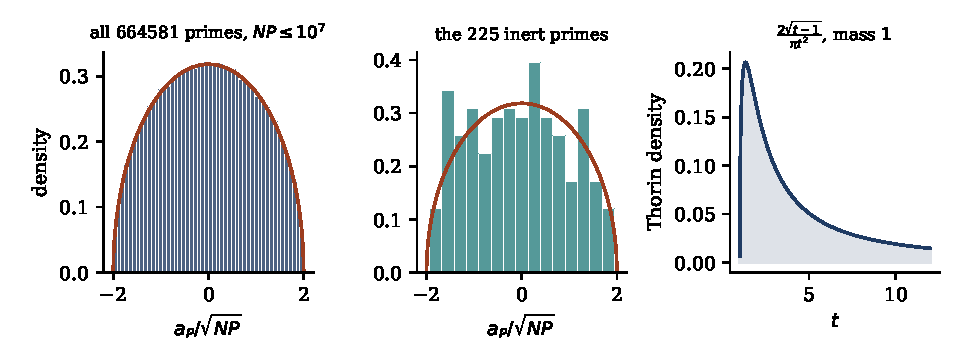
\includegraphics[width=\textwidth]{figs/cal_cm.pdf}
\caption{Sato Tate over $\Q(i)$ for $y^2=x^3+ix+1$. Left: the normalised Frobenius traces at the $664581$ primes of norm at most $10^7$ against the Sato Tate density. Centre: the $225$ inert primes alone. Right: the Thorin density $\frac2{\pi t^2}\sqrt{t-1}$ of the limiting Frobenius functional $\Xi(\cos^2)$ of Theorem~\ref{thm:calcm}, which is the same over every CM field.}\label{fig:calcm}
\end{figure}

The Ramanujan statement of Theorem~\ref{thm:calcmfield} has a local Thorin reading. A cuspidal automorphic representation of $\GL_2(\A_F)$ of weight zero over an imaginary quadratic $F$ is a Bianchi modular form, the analogue over $F$ of a holomorphic form of weight two, and its Hecke eigenvalues $\lambda(\mathfrak p)=\alpha_{\mathfrak p}+\alpha_{\mathfrak p}^{-1}$ at unramified primes were not known to satisfy $|\lambda(\mathfrak p)|\le2$ before \cite{accghlnstt2023}, Deligne's theorem not applying because the forms are not holomorphic in any sense and the locally symmetric space is a hyperbolic three manifold rather than a Shimura variety.

\begin{corollary}[local Thorin positivity for Bianchi forms]\label{cor:calbianchi}
Let $\pi$ be a cuspidal automorphic representation of $\GL_2(\A_F)$ of weight zero, $F$ a CM field, and $\mathfrak p$ an unramified prime at which the central character is trivial, with Satake parameters $\alpha_{\mathfrak p}^{\pm1}$ and $\lambda(\mathfrak p)\ne2$. Then, in the variable $u$ of the Laplace transform, $(2-\lambda(\mathfrak p))N\mathfrak p^{-\sqrt u}L_{\mathfrak p}(\sqrt u,\pi)$ is the Laplace transform of a GGC with Thorin comb $\sum_{k\in\Z}\delta_{((\theta_{\mathfrak p}+2\pi k)/\log N\mathfrak p)^2}$, $\lambda(\mathfrak p)=2\cos\theta_{\mathfrak p}$, unconditionally.
\end{corollary}

\begin{proof}
Theorem~\ref{thm:10clocal} with $x=\lambda(\mathfrak p)$ and $L=\log N\mathfrak p$, the hypothesis $-2\le x<2$ being Theorem~\ref{thm:calcmfield}.
\end{proof}

This is the local positivity that Corollary~\ref{cor:msramanujan} states conditionally for Maass forms over $\Q$, here proved for the weight zero forms over CM fields. Over $\Q$ and over totally real fields the weight zero forms are the holomorphic forms of weight two and the bound is Eichler, Shimura and Igusa's, through the Shimura variety; over a CM field the locally symmetric space is not algebraic and no such route exists, which is why the bound was open there until \cite{accghlnstt2023}, whose proof goes through the potential automorphy of every symmetric power and the theorem of Jacquet and Shalika. The Maass forms of eigenvalue $\frac14$ over $\Q$ have the infinitesimal character of weight one, are not cohomological, and remain out of reach of both routes.

\section{Abelian surfaces: the Thorin criterion made well posed}\label{sec:calg2}

The Thorin equivalence theorem, Theorem~\ref{thm:10bmain}, needs an $L$ function that is entire of finite order with a functional equation; it is stated for automorphic $L$ functions, where Godement and Jacquet supply these properties, and its probabilistic content is that GRH is membership in the GGC class. For the $L$ function of an abelian surface $A/\Q$, of degree four with gamma factor $\Gamma_\C(s)^2$ in the motivic normalisation, the properties were conjectural before Theorem~\ref{thm:calbcgp}, which supplies meromorphic continuation and the functional equation for every $A$, and, for the modular ones, holomorphy by Godement and Jacquet.

\begin{theorem}[Thorin criterion for abelian surfaces]\label{thm:calg2}
Let $A/\Q$ be an abelian surface with $\operatorname{End}_{\C}(A)=\Z$, $\Lambda(s,A)=N_A^{s/2}\Gamma_\C(s)^2L(s,A)$, and suppose $\Lambda(s,A)$ is entire, as it is for the modular surfaces, where Godement and Jacquet supply it, and is expected for all. Put $\Xi_A(w)=\Lambda(1+w,A)$, even, with zeros $\pm i\gamma_k$ written as $1\pm i\gamma_k$ in $s$, and suppose $\Lambda(1,A)\ne0$. Then GRH for $A$ holds if and only if $\Xi_A(0)/\Xi_A(\sqrt\lambda)$ is the Laplace transform of a GGC, in which case the Thorin measure is $\sum_k\delta_{\gamma_k^2}$ and the GGC is $\sum_kE_k/\gamma_k^2$; and for every basepoint $1+a$ with $a\ge\frac12$ the shifted representation of Theorem~\ref{thm:10dshift} holds unconditionally.
\end{theorem}

\begin{proof}
With the functional equation $\Lambda(s,A)=\pm\Lambda(2-s,A)$, root number $+1$ when $\Lambda(1,A)\ne0$, and holomorphy of finite order, $\Xi_A$ is even and entire of order one, since the Brauer induction of the potential modularity argument writes $\Lambda(s,A)$ as a ratio of products of automorphic $L$ functions, each entire of order one, and the proof of Theorem~\ref{thm:10bmain} applies verbatim; the zero counting function is $O(T\log T)$, so the Thorin measure $\sum\delta_{\gamma_k^2}$ satisfies the integrability conditions. The shifted representation is Theorem~\ref{thm:10dshift}(iii), whose hypothesis is that all zeros have $|\operatorname{Re}(s-1)|<\frac12$, which is the nonvanishing of $L(s,A)$ on $\operatorname{Re}s\ge\frac32$: on $\operatorname{Re}s>\frac32$ from the absolutely convergent Euler product, and on the line $\operatorname{Re}s=\frac32$ from potential automorphy, Brauer induction and the theorem of Jacquet and Shalika.
\end{proof}

For the curve $C:y^2+(x^3+1)y=x^2+x$ of conductor $249$, the smallest conductor of a genus two curve over $\Q$ whose Jacobian has endomorphism ring $\Z$ \cite{lmfdb}, whose modularity is expected but not among the cases proved, so that holomorphy of $\Lambda(s,C)$ is assumed in what follows, the $L$ function was computed by PARI and its zeros found to height $T$; the counting function $\frac{4T}{2\pi}\log\frac T{2\pi e}+\frac T{2\pi}\log249$ predicts their number to within one. The product $\prod_k(1+\lambda/\gamma_k^2)$ over these zeros with the tail from the counting function reproduces $\Xi_C(\sqrt\lambda)/\Xi_C(0)$ as stated in Table~\ref{tab:calg2} and Figure~\ref{fig:calg2}; the agreement improves with $T$ as the tail approximation does, and nothing in the data is inconsistent with the Thorin measure being $\sum\delta_{\gamma_k^2}$, which is GRH for $C$. The normalised traces $a_p/\sqrt p$ of Frobenius at the primes of good reduction among the first $20000$ primes ($19997$ of them) have moments as in Table~\ref{tab:calg2} against the moments $1$, $3$, $14$ of the trace of a Haar distributed element of $\USp(4)$, the Sato Tate group of a generic abelian surface; Sato Tate for abelian surfaces with endomorphism ring $\Z$ remains open, potential modularity of the symmetric powers being out of reach, while the other Sato Tate groups are settled, so these moments are a conjecture checked, not a theorem illustrated.

\begin{table}[t]
\centering\small
\begin{tabular}{@{}rrrr@{}}
\toprule
$\lambda$ & $\Xi_C(\sqrt\lambda)/\Xi_C(0)$ & product over zeros & relative error\\
\midrule
$0.25$ & $1.08273$ & $1.08272$ & $1.1\cdot10^{-5}$\\
$1$ & $1.37192$ & $1.37186$ & $4.4\cdot10^{-5}$\\
$4$ & $3.45361$ & $3.453$ & $1.8\cdot10^{-4}$\\
$9$ & $14.9836$ & $14.9777$ & $4.0\cdot10^{-4}$\\
$16$ & $104.024$ & $103.95$ & $7.1\cdot10^{-4}$\\
$36$ & $15805.4$ & $15780.3$ & $1.6\cdot10^{-3}$\\
\bottomrule
\end{tabular}
\caption{The Thorin product of the genus two curve of conductor $249$, from the 101 zeros below height $60$ and the tail integral. Frobenius moments of $a_p/\sqrt p$ at the primes of good reduction among the first $20000$ primes ($19997$ of them): $1.002$, $2.982$, $13.81$ against $1$, $3$, $14$ for $\USp(4)$.}\label{tab:calg2}
\end{table}

\begin{figure}[t]
\centering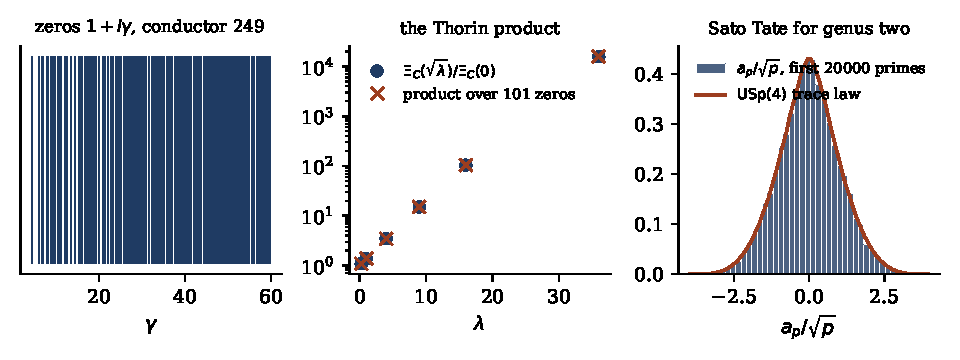
\includegraphics[width=\textwidth]{figs/cal_g2.pdf}
\caption{The genus two curve of conductor $249$. Left: the zeros $1+i\gamma$ of $\Lambda(s,C)$ below height $60$, the atoms $\gamma^2$ of its Thorin measure if GRH holds. Centre: $\Xi_C(\sqrt\lambda)/\Xi_C(0)$ against the product over the zeros. Right: the normalised Frobenius traces at the primes of good reduction among the first $20000$ primes ($19997$ of them) against the trace density of $\USp(4)$.}\label{fig:calg2}
\end{figure}

What Theorem~\ref{thm:calbcgp} changes is the status of the question. Before it, the GGC property of $\Xi_A(0)/\Xi_A(\sqrt\lambda)$ was a statement about a function not known to exist beyond $\operatorname{Re}s>\frac32$; after it, the function exists, is even, and the Thorin criterion is a precise conjecture that can be tested at every zero. The same remark applies to the whole of Chapters~\ref{ch:10b} to \ref{ch:10d} for abelian surfaces, and in particular to the computational programme of Chapter~\ref{ch:14}, whose Hankel and Stieltjes tests can now be run on genus two $L$ functions with the knowledge that the object tested is well defined.

\section{Torsion and entropy}\label{sec:caltorsion}

The Taylor Wiles method identifies a deformation ring with a Hecke algebra acting on the cohomology of a modular curve, which is torsion free. For $\GL_2$ over an imaginary quadratic field the locally symmetric space is a hyperbolic three manifold, its first homology has torsion, and Bergeron and Venkatesh \cite{bergeronvenkatesh2013} conjectured that the torsion grows exponentially in the volume,
\begin{equation}\label{eq:calbv}
\frac{\log|H_1(\Gamma_N,\Z)_{\mathrm{tors}}|}{\operatorname{vol}(\Gamma_N\backslash\mathbb H^3)}\longrightarrow\frac1{6\pi}
\end{equation}
for $\Gamma_N$ running through principal congruence subgroups of an arithmetic lattice in $\SL_2(\C)$, and proved the analogous limit, with a constant $c_{G,M}$, for strongly acyclic coefficient modules $M$ over cocompact arithmetic lattices; trivial coefficients, and the Bianchi groups, which are not cocompact, remain conjectural. The constant $\frac1{6\pi}$ is, up to sign, the $L^2$ torsion of hyperbolic three space per unit volume. Calegari and Venkatesh \cite{calegarivenkatesh2019} showed that this torsion obeys a Jacquet Langlands correspondence: the torsion in the homology of the quotient by a unit group of a quaternion algebra over $F$ matches, in a precise sense, torsion in the homology of the split group, with the discrepancies explained by congruences. The method of Calegari and Geraghty is what makes torsion classes usable for modularity lifting.

The book met a statement of the shape \eqref{eq:calbv} in Chapter~\ref{ch:hit}. Theorem~\ref{thm:hitentropy} says that for a fixed prime $\ell$ and $N\to\infty$ through primes
\[
\frac1g\log|J_0(N)(\mathbb F_\ell)|\longrightarrow\log\frac{\ell^\ell}{(\ell^2-1)^{(\ell-1)/2}},
\]
the spanning tree entropy of the $(\ell+1)$ regular tree, with $g$ the genus of $X_0(N)$, and that the bridge between the two sides is the Jacquet Langlands correspondence between $J_0(N)$ and the supersingular isogeny graph in characteristic $N$, whose number of spanning trees is $|J_0(N)(\mathbb F_\ell)|$ divided by the rational torsion. The analogy with \eqref{eq:calbv} is exact in shape: a count of points modulo $\ell$, or of torsion, grows exponentially in the volume, with a constant that is the entropy of a random walk on the universal cover, the tree in one case and hyperbolic three space in the other, and the Jacquet Langlands correspondence transports the count between the split and the quaternionic side. In the tree case the constant is the growth rate of the number of spanning trees per vertex, $\log\ell^\ell/(\ell^2-1)^{(\ell-1)/2}$, which Lyons calls the tree entropy; in the hyperbolic case it is the $L^2$ analytic torsion, which is the regularised determinant of the Laplacians on forms and is computed from the heat traces of Chapter~\ref{ch:maass} in dimension three, $\log T^{(2)}=\frac12\sum_j(-1)^jj\,\zeta'_j(0)$ with $\zeta_j(s)=\Gamma(s)^{-1}\int_0^\infty t^{s-1}\operatorname{tr}e^{-t\Delta_j}\,dt$ regularised. Both constants are return probabilities of Brownian motion or of random walk on the universal cover, integrated against time. The precise relation is Open Problem~\ref{op:caltorsion}.

\section{What this adds to the programme}

The chapter adds one theorem and three transfers. Theorem~\ref{thm:calparity} extends the comparison of gamma factors of Section~\ref{sec:msquarter} from weight one to every weight, with the law $C+\frac w2T$ in place of the secant law, and reads Calegari's theorem on even representations as the statement that for distinct Hodge Tate weights the archimedean term of the heat trace is never the even one. Theorem~\ref{thm:calcm} and Corollary~\ref{cor:calbianchi} transfer the Dirichlet process and the local Thorin positivity to CM fields, where the theorems of Calegari and his coauthors make the hypotheses of Chapters~\ref{ch:recip} and \ref{ch:pd} theorems. Theorem~\ref{thm:calg2} transfers the Thorin criterion to abelian surfaces, where it is now a well posed conjecture rather than a statement about a function of unknown existence. Section~\ref{sec:caltorsion} records that the entropy theorem of Chapter~\ref{ch:hit} and the torsion growth of Bergeron and Venkatesh have the same shape, and leaves the identification of the constants open.

\section{Notes}

The theorems quoted are \cite{calegari2011,calegari2012,calegarigeraghty2018,accghlnstt2023,bcgp2021,calegarivenkatesh2019,bergeronvenkatesh2013}; the Fontaine Mazur conjecture is \cite{fontainemazur1995} and Ramakrishna's even representations are \cite{ramakrishna2002}. The Sato Tate theorem over totally real fields is \cite{blght2011}. The genus two $L$ function and its zeros were computed with PARI \cite{pari2023} (\texttt{lfungenus2}, \texttt{lfunzeros}, \texttt{hyperellcharpoly}); the curve is $249.a.249.1$ in the LMFDB \cite{lmfdb}. The identity $\psi(\frac{z+1}2)-\psi(\frac z2)=2\int_0^\infty e^{-zu}(1+e^{-u})^{-1}du$ is the standard integral representation of the digamma function, and the Fourier transform of the hyperbolic secant is classical. Theorems~\ref{thm:calparity}, \ref{thm:calcm} and \ref{thm:calg2} and Corollary~\ref{cor:calbianchi} are new as formulated; each is a consequence of the cited theorems and of Chapters~\ref{ch:10b}, \ref{ch:10c}, \ref{ch:10d}, \ref{ch:recip}, \ref{ch:flt} and \ref{ch:pd}.

\section{Exercises}

\begin{enumerate}
\item Show that $f_w(0)=\int_\R\operatorname{sech}(\pi s)\frac{w/2\pi}{(w/2)^2+s^2}\,ds$ decreases from $1$ to $0$ and that $f_w(0)\sim2/(\pi w)$ as $w\to\infty$; check against $0.0574$ at $w=11$, where $2/(11\pi)=0.0579$.
\item Prove that the density of $C_w$ is log concave for $w=0$ and, having Cauchy tails, for no $w>0$.
\item For a weight $k$ newform $f$ with a zero of order $m$ at the centre, show under GRH that $\mathcal W^{\mathrm{hol}}_f(x)\to\frac m2$ and that $\mathcal W^{\mathrm{ev}}_f$ still fails to be completely monotone; note that the functional equation of Theorem~\ref{thm:calparity} must be read with the root number $(-1)^m$.
\item Show that for an elliptic curve $E/\Q$ without complex multiplication and any CM field $F$, the Dirichlet process of Theorem~\ref{thm:calcm} over $F$ has the same base measure as over $\Q$, and compute the Mertens constants of the classes $\{\theta_{\mathfrak p}\in A\}$ in terms of the symmetric power $L$ functions over $F$.
\item Write the Thorin comb of Corollary~\ref{cor:calbianchi} for a Bianchi form over $\Q(\sqrt{-1})$ of level $(1+i)^k$ taken from the LMFDB at the primes of norm $5$ and $9$.
\item Show that for an abelian surface over $\Q$ with real multiplication defined over $\Q$ the $L$ function is $L(s,f)L(s,f^\sigma)$ for a weight two newform $f$ with coefficients in a real quadratic field and its conjugate, and that the Thorin measure of the degree four function is the sum of the two degree two Thorin measures of Chapter~\ref{ch:10b}; when the real multiplication is defined only over a real quadratic field $K$, show that $L(s,A)=L(s,E/K)$ for an elliptic curve $E/K$.
\item Verify the counting function $\frac{4T}{2\pi}\log\frac T{2\pi e}+\frac T{2\pi}\log N$ for the zeros of a degree four $L$ function with gamma factor $\Gamma_\C(s)^2$ from the argument principle.
\end{enumerate}

\section{Open problems}

\begin{problem}[parity without GRH]\label{op:calparity}
Theorem~\ref{thm:calparity}(b) shows under GRH that $\mathcal W^{\mathrm{ev}}_\rho$ fails to be completely monotone for odd $\rho$. Find an unconditional proof that at most one of $\mathcal W^{\mathrm{hol}}_\rho$ and $\mathcal W^{\mathrm{ev}}_\rho$ is completely monotone, for a self dual $\rho$ with distinct Hodge Tate weights; the difference $\Delta_w$ is completely monotone, so the question is whether a completely monotone function can differ from another by $\Delta_w$ when both are heat traces of the same Frobenius data.
\end{problem}

\begin{problem}[the Euler Kronecker drift over a CM field]\label{op:calshape}
For $E/F$ without complex multiplication, $F$ a CM field, the Rankin Selberg subordinator of Section~\ref{sec:recipgalois} over $F$ has Gamma shape $1$, since $L(s,\rho|_F\otimes\check\rho|_F)=\zeta_F(s)L(s,\operatorname{ad}^0\rho|_F)$ and the second factor is holomorphic and nonzero at $s=1$ by \cite{accghlnstt2023}, Brauer induction and Jacquet and Shalika. Determine the Euler Kronecker drift of Theorem~\ref{thm:recipdrift} over $F$ in terms of the Euler Kronecker constant of $F$ and $L'/L(1,\Sym^2E/F)$, and its dependence on the degree of $F$; and decide whether the deficits of the Sato Tate classes can change sign with the field.
\end{problem}

\begin{problem}[Sato Tate for abelian surfaces as a Dirichlet process]\label{op:calg2}
State the Sato Tate conjecture for a generic abelian surface over $\Q$ in the form of Theorem~\ref{thm:calcm}, with base measure the law of the trace of a Haar distributed element of $\USp(4)$, and determine which Frobenius functionals have Gamma limits that are provable from Theorem~\ref{thm:calbcgp} alone, that is from the Rankin Selberg $L$ function and the standard $L$ function of $\mathrm{GSp}_4$ without symmetric powers.
\end{problem}

\begin{problem}[torsion entropy and tree entropy]\label{op:caltorsion}
Identify the constant $\frac1{6\pi}$ of \eqref{eq:calbv} as an entropy of a random walk or Brownian motion on hyperbolic three space in the sense in which $\log\ell^\ell/(\ell^2-1)^{(\ell-1)/2}$ is the spanning tree entropy of the $(\ell+1)$ regular tree in Theorem~\ref{thm:hitentropy}, and find the common statement of which the two are the $p$ adic and the archimedean cases: a Jacquet Langlands invariant growth rate of torsion, computed from return probabilities on the universal cover.
\end{problem}

\begin{compproblem}[genus two Thorin tests]\label{cp:calg2}
Objective: for the $66158$ genus two curves of discriminant below $10^6$ in the LMFDB, compute the first $50$ zeros of $\Lambda(s,C)$, test the Thorin product and the Hankel criterion of Chapter~\ref{ch:14} at the basepoints $1$, $\frac32$ and $2$, and record the margins; compute the Frobenius moments at the primes below $10^6$ for the curves with $\operatorname{End}=\Z$ against $\USp(4)$ and for the curves with real multiplication defined over $\Q$ against the law of the sum of two independent $\SU(2)$ traces. Starting point: \texttt{c3.py}.
\end{compproblem}
